% Original vector reconstruction: source Fig.45.1, PDF194 / printed182.
% Five diagrams: (a) fermion and scalar free terms; (b), (c), (d).
% Large dots are sources; small dots are Yukawa vertices.
% Fermion arrows: eta -> bar eta. Scalar coordinate lines have no arrows.
% Basic TikZ only. No figure environment, caption, or automatic numbering.
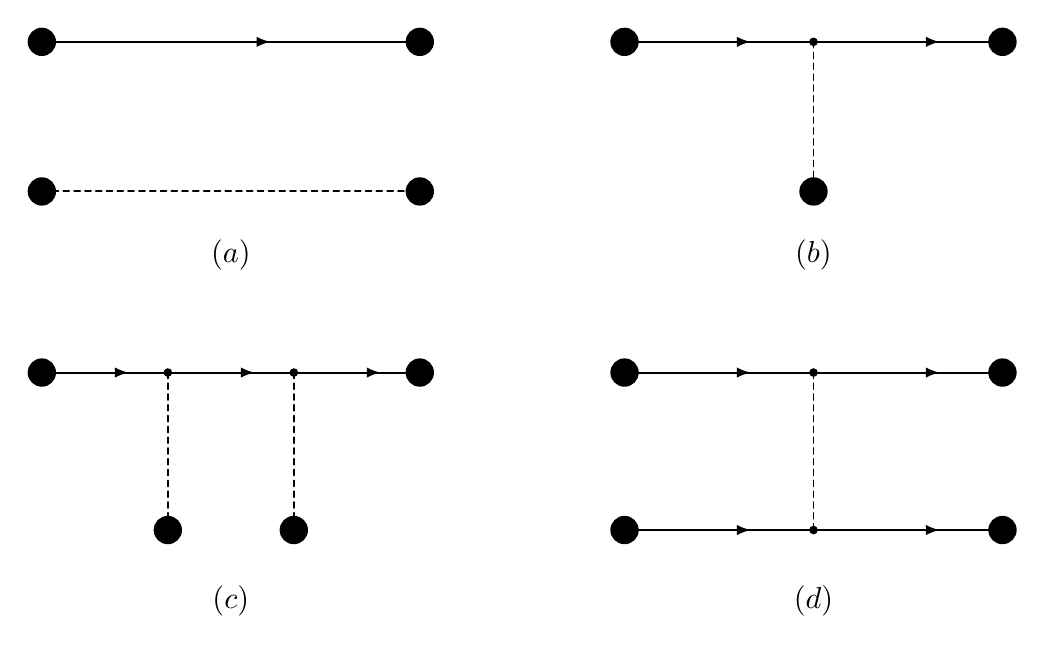
\begin{tikzpicture}[x=1mm,y=1mm,line width=.7pt,>=latex,
  line cap=round,line join=round,font=\fontsize{10.5}{12}\selectfont,
  scalar/.style={dash pattern=on 2.1pt off 1.8pt}]
  % (a): two separate connected free diagrams.
  \draw (0,10)--(48,10);
  \draw[->] (18,10)--(29,10);
  \draw[scalar] (0,-9)--(48,-9);
  \foreach \x in {0,48}{
    \fill (\x,10) circle[radius=1.8mm];
    \fill (\x,-9) circle[radius=1.8mm];
  }
  \node at (24,-17) {$(a)$};
  % (b): eta--V--bar eta, with V--J below.
  \draw (74,10)--(122,10);
  \draw[->] (81,10)--(90,10);
  \draw[->] (105,10)--(114,10);
  \draw[scalar] (98,10)--(98,-9);
  \foreach \x in {74,122}{\fill (\x,10) circle[radius=1.8mm];}
  \fill (98,-9) circle[radius=1.8mm];
  \fill (98,10) circle[radius=.55mm];
  \node at (98,-17) {$(b)$};
  % (c): two ordered Yukawa vertices along one open fermion chain.
  \draw (0,-32)--(48,-32);
  \draw[->] (4,-32)--(11,-32);
  \draw[->] (20,-32)--(27,-32);
  \draw[->] (36,-32)--(43,-32);
  \draw[scalar] (16,-32)--(16,-52);
  \draw[scalar] (32,-32)--(32,-52);
  \foreach \x in {0,48}{\fill (\x,-32) circle[radius=1.8mm];}
  \foreach \x in {16,32}{
    \fill (\x,-52) circle[radius=1.8mm];
    \fill (\x,-32) circle[radius=.55mm];
  }
  \node at (24,-61) {$(c)$};
  % (d): two ordered source chains joined by a scalar propagator.
  \foreach \y in {-32,-52}{
    \draw (74,\y)--(122,\y);
    \draw[->] (81,\y)--(90,\y);
    \draw[->] (105,\y)--(114,\y);
    \fill (74,\y) circle[radius=1.8mm];
    \fill (122,\y) circle[radius=1.8mm];
    \fill (98,\y) circle[radius=.55mm];
  }
  \draw[scalar] (98,-32)--(98,-52);
  \node at (98,-61) {$(d)$};
\end{tikzpicture}
